\documentclass[../relazione.tex]{subfiles}

\begin{document}
Il progetto presenta una gerarchia unica nella parte logica che rappresenta tutte le varie entità che possono essere istanziate nel gioco.
Queste entità possono essere di tipo Character oppure di tipo Item. Queste ultime due classi possiamo considerarle come classi base per altre due "sotto-gerarchie".\\
Questa libreria è stata implementata utilizzando solamente STL in modo da renderla più indipendente possibile dal framework Qt.\\
\subsection{Gerarchia Entity}

\begin{figure}[h]
    \centering
    \begin{subfigure}[b]{1\linewidth}
        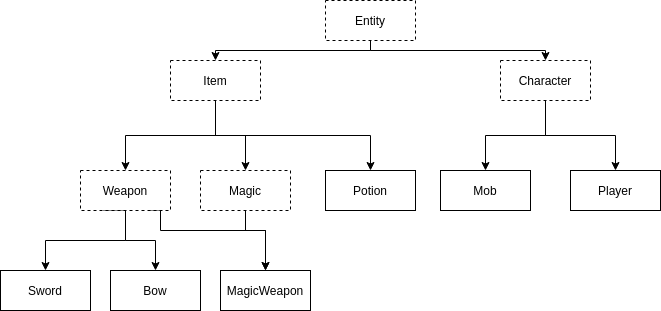
\includegraphics[width=\linewidth]{img/entity.png}
        \caption{Gerarchia Entity.}
    \end{subfigure}
    \label{fig:gerarchia-entity}
\end{figure}

Nella figura vediamo che la classe Entity che non contiene alcun attributo ed é virtuale pura.
Entity rappresenta la classe base da cui derivano quelle che possiamo definire come due "sotto-gerarchie", Character e Item.\\ \\
Character aggiunge gli attributi che un qualsiasi personaggio del gioco, sia il personaggio giocante, sia i nemici che si affronteranno, devono avere;
ovvero un nome, il numero di punti vita e punti mana, un riferimento all'arma equipaggiata ed un riferimento all'armatura equipaggiata.\\
Da Character derivano a loro volta due classi istanziabili, Mob e Player. Player implementa un attributo inventory, che rappresenta l'inventario del nostro personaggio.\\
Inventory è il container che abbiamo implementato per contenere gli oggetti (armi, armature e pozioni) in cui abbiamo definito tutti i metodi utili per la sua gestione.\\ \\
\newpage{}
Item, come Character é una classe virtuale, inoltre aggiunge l'attributo nome e un ID, variabile utile alla gestione dell'inventario.
Item contiene il metodo virtuale \textbf{use()} che permette l'utilizzo degli oggetti passandogli un riferimento al Character "utilizzatore" e uno al Character "target"; 
Da Item derivano altre tre classi, Weapon, Magic e Potion.
Weapon e Magic aggiungono l'attributo danno nella prima e gli attributi mana ed effetto nella seconda; sono entrambe virtuali pure.
La classe istanziabile Potion aggiunge l'attributo effect, che indica la quantità di punti che può ripristinare; inoltre contiene due variabili di tipo bool che indicano quale
delle due statistiche del personaggio andrá a ripristinare.
Da Weapon derivano le due classi istanziabili Sword e Bow che si concretizzano come le spade e gli archi che il personaggio e i nemici utilizzeranno.\\
Weapon aggiunge l'attributo range, mentre Bow aggiunge l'attributo frecce che indica il numero di frecce a sua disposizione, le quali ad ogni utilizzo dell'arco
verranno decrementate.
La classe istanziabile MagicWeapon rappresenta la classe che abbiamo implementato utilizzando l'ereditarietà multipla in quanto deriva sia da Magic che da Weapon.

\subsection{Classe contenitore}
\label{ssec:classe-contenitore}
La classe contenitore simula il funzionamento di una struttura vector presente in STL. Impementa tutti i vari metodi di inserimento e rimozione facendo anche utilizzo
di Iterator e Const\_Iterator.
\end{document}